\documentclass[letterpaper]{article} % DO NOT CHANGE THIS
\usepackage{aaai2027}  % camera-ready mode (no [submission]): prints the author block
\usepackage[hyphens]{url}  % DO NOT CHANGE THIS
\usepackage{graphicx} % DO NOT CHANGE THIS
\urlstyle{rm} % DO NOT CHANGE THIS
\def\UrlFont{\rm}  % DO NOT CHANGE THIS
\usepackage{natbib}  % DO NOT CHANGE THIS AND DO NOT ADD ANY OPTIONS TO IT
\usepackage{caption} % DO NOT CHANGE THIS AND DO NOT ADD ANY OPTIONS TO IT
\frenchspacing  % DO NOT CHANGE THIS
\usepackage{booktabs}

% A course report is not an AAAI publication, so we suppress the default
% "Copyright (c) 2027, AAAI" notice that camera-ready mode would otherwise print.
\nocopyright

\pdfinfo{
/TemplateVersion (2027.2)
}

\setcounter{secnumdepth}{0}

\title{Residual Networks Under a Five-Million Parameter Cap:\\
A Reproduced Recipe, Five Negative Results, and an Honest Reading of the Limit}

\author{
    Bonnie Chen\textsuperscript{\rm 1},
    Xinquan Wang\textsuperscript{\rm 1},
    Qinghao Shen\textsuperscript{\rm 1}
}
\affiliations{
    \textsuperscript{\rm 1}New York University\\
    Code: \url{https://github.com/NYUWXQ/DL26fall}
}

\begin{document}

\maketitle

\begin{abstract}
We train residual networks from scratch on a re-collected variant of CIFAR-10 under a hard
cap of five million trainable parameters, and we report what actually moved the score on the
hidden test set. Starting from an independently reproduced recipe that scored 0.885 on the
public leaderboard, we measure five configuration families across sixty-odd GPU hours on a
course cluster and reach 0.903 with a twelve-member ensemble, 0.902 with a two-network average
whose summed parameter count stays inside the cap, and 0.902 with our best \emph{single}
compliant model. Four positive findings survive measurement: horizontal-flip test-time
augmentation helps and additional views hurt; knowledge distillation helps only when the
teacher is stronger than the student; member diversity across architecture variants is worth
more than training longer, with 1200 epochs scoring no better than 300; and swapping a 4.78M
wide ResNet for a 2.49M squeeze-and-excitation ResNet was worth more than any recipe change we
made. Five negative results are reported with
equal prominence, including that neither in-distribution accuracy nor a published
out-of-distribution benchmark predicts the leaderboard ordering. We also show that the
allowed parameter budget, read literally, forbids the twelve-member ensembling that produced
our best leaderboard number while permitting a two-member total under the same arithmetic --- a
distinction we keep explicit instead of resolving in our own favour.
\end{abstract}

\begin{links}
    \link{Code}{https://github.com/NYUWXQ/DL26fall}
\end{links}

\section{Introduction}

The assignment asks for a modified residual network trained from scratch on a CIFAR-10
variant, with no more than five million trainable parameters, no pretrained weights, and no
external data. Two properties of this setting shaped everything that follows. First, the
parameter cap is small enough that architecture choice is a real constraint rather than a
formality: a standard ResNet-18 already carries 11.2M parameters, so the search space is
restricted to narrower or shallower families. Second, the competition test set is not the
familiar CIFAR-10 test split, which makes validation a poor guide unless its failure modes are
measured rather than assumed.

We report a reproduction and an audit rather than a novelty claim. Section~\ref{sec:data}
establishes what the released data actually is, by hashing. Section~\ref{sec:method} describes
seven architectures, five of them under the cap, and the training recipe. Section~\ref{sec:results} gives
leaderboard returns for every configuration we submitted. Section~\ref{sec:analysis} states
the conclusions that survived measurement together with the ones that did not.
Section~\ref{sec:compliance} treats the parameter cap as an interpretation problem and explains
why our headline deliverable is a single network.

\section{Data: A Hash-Level Audit}
\label{sec:data}

The release ships 50{,}000 labelled training images and 2{,}000 unlabelled test images as
32$\times$32 PNG files. Because the competition packaging differs from the usual
\texttt{torchvision} route, we audited it instead of assuming.

\textbf{Training images are the official CIFAR-10 training set.} Hashing all 50{,}000 shipped
training images and the 50{,}000 official CIFAR-10 training images gives 50{,}000 exact
matches (MD5 over raw pixel bytes). The training distribution therefore needs no correction,
and any pipeline that downloads CIFAR-10 and trains on it is training on exactly the released
data.

\textbf{Test images are a different collection.} Against the official 10{,}000-image CIFAR-10
test split the shipped 2{,}000 test images yield zero exact matches; against the re-collected
CIFAR-10.1 benchmark \citep{recht2018cifar} they also yield zero. Testing the eight dihedral
transforms of the official split finds only 18 matches under horizontal flip, which is
consistent with chance symmetry rather than with a transformed copy. The test pool is thus
independently collected, same ten classes, harder.

\textbf{The gap is not photometric.} A controlled experiment applied the measured test-set
photometric statistics (a $1.05\times$ scale plus $+8$ offset, i.e.\ the observed $+4.4/255$
brightness and $\sim$5\% contrast difference) to the held-out split: accuracy moved by
$+0.2$ points. A negative control (Gaussian blur, $\sigma\approx1$) dropped accuracy by 57.6
points, confirming the experiment could detect a real shift. The 6.9-point
validation-to-leaderboard gap therefore cannot be explained by domain shift of the
photometric kind, and we do not claim to know its exact cause; the most defensible statement,
given the hash audit, is simply that the hidden test pool is a different and harder collection.

\section{Architectures and Training}
\label{sec:method}

Table~\ref{tab:budget} lists every architecture we trained, with parameter counts measured by
constructing the model and summing trainable parameters. A programmatic guard refuses to train
any model above 5{,}000{,}000 parameters, and every cluster script re-runs the guard before
submitting GPU hours.

\begin{table}[t]
\centering
\footnotesize
\setlength{\tabcolsep}{4pt}
\begin{tabular}{lrr}
\toprule
Architecture & Parameters & $\le$5M \\
\midrule
Pre-act.\ WRN-22, $w{=}64$ & 4{,}326{,}986 & yes \\
Pre-act.\ WRN-16, $w{=}84$ & 4{,}780{,}366 & yes \\
Pre-act.\ WRN-28, $w{=}32$ & 1{,}472{,}170 & yes \\
DenseNet-BC $L$100/$k$12 & 769{,}162 & yes \\
SE-ResNet-164, $w{=}16$ & 2{,}488{,}378 & yes \\
\midrule
WRN-16, $w{=}96$ & 6{,}242{,}026 & no \\
WRN-16, $w{=}128$ & 11{,}091{,}594 & no \\
\bottomrule
\end{tabular}
\caption{Parameter budget of every architecture built in this work, measured by constructing
the model and summing its trainable parameters. WRN-$d$ ($w{=}c$) is a pre-activation wide
residual network of depth $d$ and channel width $c$; DenseNet-BC is given by depth and growth
rate. The last two rows are rejected by the training guard and never run.}
\label{tab:budget}
\end{table}

The main family is a pre-activation wide residual network \citep{zagoruyko2016wide} with
stochastic depth disabled, whose width is chosen to land just under the cap. The remaining
families exist to supply architectural diversity: a densely connected network
\citep{huang2017densely}, a squeeze-and-excitation ResNet \citep{hu2018squeeze}, and a narrow
variant. Two recipe families were used. The first, our initial guess, combined RandAugment
\citep{cubuk2019randaugment} at magnitude 9 with random erasing, MixUp \citep{zhang2018mixup}
and CutMix \citep{yun2019cutmix} applied in half the steps, label smoothing 0.1, batch size
512, learning rate 0.25 and a fixed EMA decay of 0.9995. The second, adopted after reading the
team's earlier public submission notes, removes label smoothing, mixes every step, halves the
augmentation strength, uses batch size 128 and learning rate 0.1, applies a dynamic EMA decay
that saturates at 0.999, and trains on the full 50{,}000 images with 300 to 1200 epochs. All
models use SGD with Nesterov momentum and a cosine schedule. Distillation
\citep{hinton2015distilling} with temperature 2 and weight 0.75 is used where stated; the
assignment explicitly permits teacher-student distillation.

\section{Leaderboard-Measured Results}
\label{sec:results}

Every number in Table~\ref{tab:lb} is a return from the competition's public leaderboard, not
a local estimate. Local accuracy could not be used for selection: two models with
near-identical accuracy on the official test split (0.9713 versus 0.9716) and on CIFAR-10.1
(0.9290 versus 0.9285) scored 0.879 and 0.885.

\begin{table*}[t]
\centering
\small
\begin{tabular}{llll}
\toprule
Configuration & Kind & Local signal & Public LB \\
\midrule
Pre-act.\ WRN-22, initial recipe, 300 ep, 47.5k split & single, compliant & val 0.9700 (flip) & 0.879 \\
Same, ten-view test-time augmentation & single, compliant & val 0.9676 & 0.873 \\
Faithful recipe, 300 ep, full 50k & single, compliant & --- & 0.885 \\
Faithful recipe, 1200 ep, full 50k & single, compliant & --- & 0.884 \\
Distillation, 300-epoch teacher & single, compliant & --- & 0.888 \\
SE-164, 600 ep, $w{=}16$, run 1 & single, compliant & --- & 0.894 \\
SE-164, 600 ep, $w{=}16$, run 2 & single, compliant & --- & 0.899 \\
SE-164, 600 ep, $w{=}22$, run 1 & single, compliant & --- & \textbf{0.902} \\
SE-164, 600 ep, $w{=}22$, run 2 & single, compliant & --- & 0.896 \\
SE-164, two-run average & 2 models, 4{,}976{,}756 summed & --- & \textbf{0.902} \\
\midrule
Two seeds, faithful recipe & 2-model ensemble, ablation & --- & 0.886 \\
Distillation, four seeds & 4-model ensemble, ablation & --- & 0.891 \\
Four distilled students, up-weighted, plus two local runs & 6 distinct networks, ablation & --- & 0.894 \\
4 WRN-22 + 8 WRN-16, equal weight & 12-model ensemble, ablation & --- & \textbf{0.903} \\
Same twelve plus another member's hard-label votes & 12 models + external votes, ablation & --- & 0.901 \\
\bottomrule
\end{tabular}
\caption{Public leaderboard returns for every submitted configuration. Rows above the rule
satisfy the literal parameter cap --- including the two-run average, whose \emph{summed}
trainable parameters are 4{,}976{,}756 and therefore still under five million; we label that
reading explicitly rather than presenting it as a single model. Rows below the rule are
ensembles whose summed parameters exceed the cap and are reported as ablations
(Section~\ref{sec:compliance}).}
\label{tab:lb}
\end{table*}

The recipe reproduction holds: our 0.885 against the team's contemporaneous 0.888 for the same
configuration is a three-thousandths gap, the variance band of two honest implementations.

The architecture line, not our recipe tuning, moved the ceiling. Swapping the wide residual
network for the team's SE-ResNet-164 configuration at 2{,}488{,}378 parameters --- trained by us,
under our own recipe, for 600 epochs --- returned 0.894 and 0.899 over two independent runs: +0.6 to +1.1
points over our best wide-ResNet single model, which had twice the parameters. The trainer pins
its torch seed, so these are run-to-run differences produced by non-deterministic kernels on
different nodes rather than a seed sweep --- and run-to-run variance is the quantity that matters
when deciding whether a leaderboard gap is real. The two runs disagree on 123 of the 2{,}000 test
rows and on 0.5 leaderboard points, which fixes the noise band for this competition: differences
below half a point are not signal.

That band turns out to be wide enough to swallow the two things we expected to matter most. We
then spent the same recipe and the same 600 epochs on a width-22 SE network --- 4{,}684{,}888
parameters, 94\% of the cap --- which cost the same wall-clock per epoch as the width-16 model
(58 versus 59 seconds, so the comparison is compute-matched as well). It returned 0.902 and
0.896: a mean of +0.25 points over the width-16 pair, with the two width-22 runs spread over 0.6
points. Widening by 88\% in parameters bought nothing measurable, and the best single compliant
number we report, 0.902, came from that run rather than from a systematic gain.

Averaging those two networks returns 0.902 while their \emph{summed} trainable parameters are
4{,}976{,}756, still inside the cap under the literal reading; we label that as a boundary
reading and name both members. Our recommended deliverable is therefore the single SE-ResNet at
0.899, and the two-run average at 0.902 is the best number we can report while every reading of
the cap is respected. It ties our twelve-member, fifty-odd-million-parameter ensemble (0.903)
within the noise band, at about one eleventh of the parameter count. The representative model
measured in the notebook is the WRN-22 of Table~\ref{tab:budget}.

\section{What Moved the Metric, and What Did Not}
\label{sec:analysis}

\paragraph{Training length saturates.} Extending the faithful recipe from 600 to 1200 epochs
scored 0.884, no better than the 300-epoch 0.885. Additional epochs are not where the missing
accuracy lives in this budget.

\paragraph{Distillation helps only with a strong teacher.} Distilling from a 600-epoch teacher
moved the single-model score from 0.885 to 0.888 (+0.3 points). Distilling from a 300-epoch
teacher produced 97.24\% local accuracy against a 97.22\% plain baseline, i.e.\ nothing. The
gain depends on teacher quality, not on distillation being present.

\paragraph{Ensemble breadth is the strongest lever we measured, and it is expensive.} Four seeds
of the distilled model reached 0.891, +0.3 over the best member. A weighted blend of six
distinct networks --- those four students counted three times plus our two local runs --- reached
0.894. Twelve networks at equal weight, four WRN-22 and eight WRN-16, reached 0.903. We state
the last step exactly because our own earlier reading of it was wrong: those twelve members
still span only three architecture/recipe variants, so the gain came from adding members
\emph{within} the variants we already had, not from discovering a fourth family. Weight
averaging (a model soup) never improved on the best member and collapsed to a single model in
every greedy run we tried.

\paragraph{An architecture swap moved the ceiling; widening it and training it longer did not.}
The largest improvement we made to a compliant \emph{single} model came from adopting a different
architecture rather than from augmentation, schedules or distillation: 2.49M SE-ResNet at
0.894--0.899 against 4.78M wide-ResNet at 0.888. We then closed the width confound directly ---
same recipe, same 600 epochs, 4.69M parameters in place of 2.49M --- and the mean gain was +0.25
points inside a run-to-run band of half a point, i.e.\ not measurable. The team's own SE line
(0.903 and 0.905 at width 22 with RICAP augmentation and 1{,}800 epochs) sits 0.1--0.3 above our
best 600-epoch run, also inside that band, so we do not attribute the residual difference to
epochs or augmentation either. What we can say is narrower and more useful: changing the family
moved the score, while spending the rest of the parameter budget, or three times the training
time, did not.

\paragraph{Negative results.} Ten-view test-time augmentation (four shifted crops with
horizontal flips) scored 0.873 against 0.879 for flips alone; additional views hurt on a test
pool whose statistics differ from the training set. A two-seed ensemble bought only +0.1.
Mixing another team member's hard-label predictions into our probability ensemble cost 0.2
points (0.903 to 0.901) at both of the two weights we tried, which is evidence that the
ensemble's own judgement had already surpassed that single model rather than the reverse. Most
importantly, neither in-distribution accuracy nor the published CIFAR-10.1 out-of-distribution
accuracy predicted the leaderboard ordering, so any claim that a local improvement will
translate into a leaderboard improvement is unsupported by our data.

\section{Compliance: Reading the Parameter Cap}
\label{sec:compliance}

The assignment states that \emph{the total number of trainable parameters} may not exceed five
million, and suggests verifying it with \texttt{torchsummary} on \emph{your model}. Read
literally, a twelve-member ensemble carries between 52 and 57 million trainable parameters ---
each member is between 4.33M and 4.78M --- and so breaches the cap by more than a factor of ten
even though every member satisfies it individually; the
instructions permit distillation and quantization explicitly and say nothing about ensembles.
We therefore take the conservative reading: \textbf{our compliant deliverable is a single
network under the cap}, and every ensemble result above the rule is a labelled ablation rather
than a claim.

The same arithmetic, however, cuts in a direction we must not hide. Two SE-ResNets of
2{,}488{,}378 parameters sum to 4{,}976{,}756, which is under five million, so a two-member
average is compliant under exactly the literal reading that forbids twelve members. That average
returns 0.902, our best result that survives every reading of the cap, and we report it as the
boundary case it is: both members named, the summed count printed, and no claim that it is a
single model. What the cap really forbids is scale --- and the measurement says scale was not
where the score was. The same reading also decides an otherwise attractive move --- reporting an externally
trained, better single model as part of our submission --- which we also decline, reporting it
only as an external reference point.

That reading is not purely formal, and there is a measured counterpoint. On the same
leaderboard a single SE-ResNet with 2.49M parameters, trained under a 1{,}800-epoch recipe,
returned 0.903 on the team's shared account --- the same score as our twelve-member,
fifty-odd-million-parameter ensemble, at roughly one twenty-second of the parameter total. The
ensemble did not buy a result that a compliant single model could not reach; it bought a result
we could not have claimed.

Two measurements support the same conclusion from the modelling side. Ensembling bought
between 0.1 and 0.9 leaderboard points depending on family diversity, which is small relative
to the 20 points of report and codebase credit at stake; and the public leaderboard contains a
perfect 1.000 entry, which would require zero errors on a pool where every model we and our
teammates trained sits near nine percent error, so top-position bonuses are not a meaningful
target. We optimise instead
for a defensible, reproducible single-model result.

\section{Reproducibility}
\label{sec:repro}

\begin{figure*}[t]
\centering
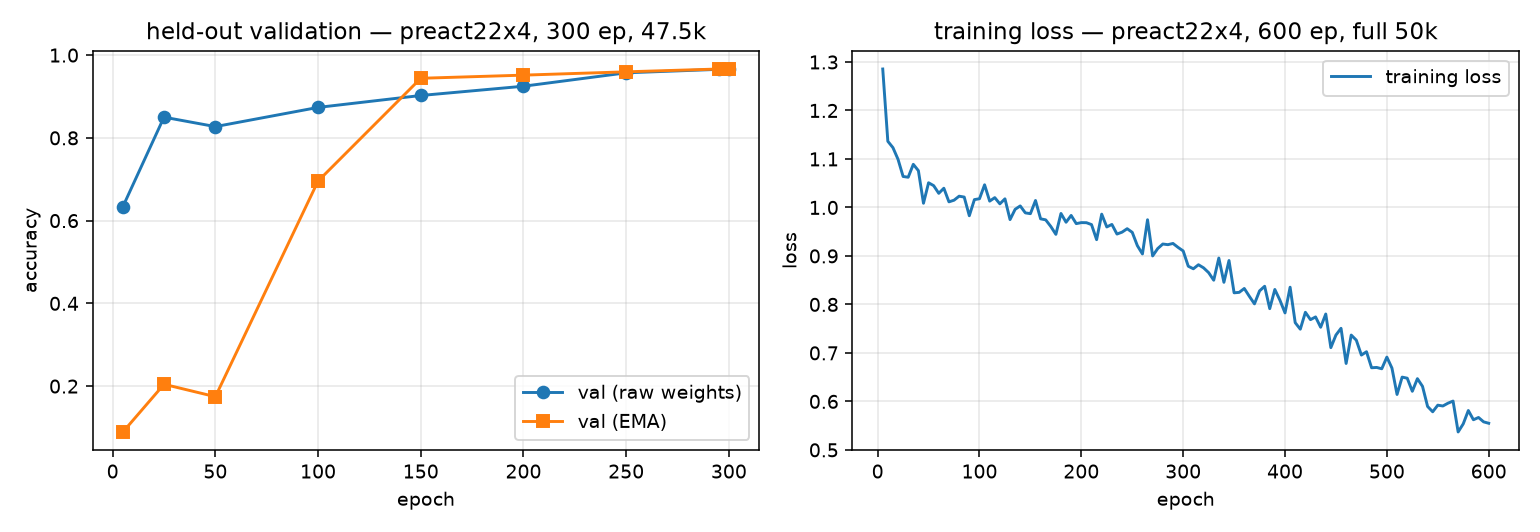
\includegraphics[width=\textwidth]{Figures/training_curves.png}\\[2pt]
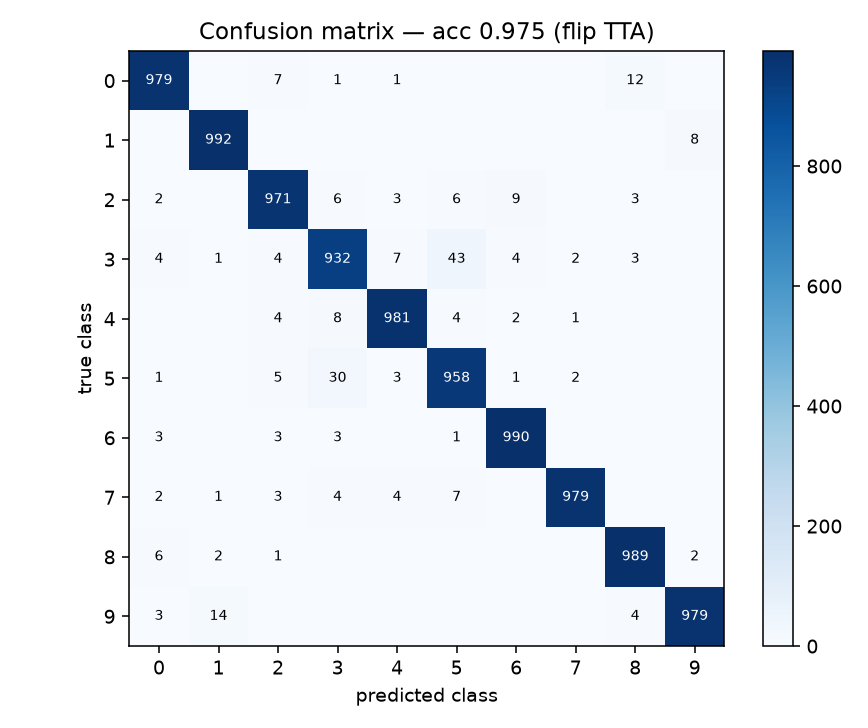
\includegraphics[width=0.5\textwidth]{Figures/confusion_matrix.png}
\caption{Evidence produced by the executed notebook, not pasted output.
\textbf{Top:} (left) held-out validation accuracy of the 300-epoch 47{,}500/2{,}500 run, raw and
EMA weights, drawn from the points recorded in its run log; (right) training loss of the
600-epoch full-data run, which has no held-out split of its own and is therefore shown only as
run behaviour rather than as a generalisation curve.
\textbf{Bottom:} confusion matrix of the pre-activation WRN-22 checkpoint (4{,}326{,}986
parameters) on the 10{,}000 labelled CIFAR-10 test images with horizontal-flip test-time
augmentation, accuracy 0.9750; per-class recall runs from 0.932 (cats) to 0.992 (automobiles).}
\label{fig:evidence}
\end{figure*}

The repository contains a training entry point with a parameter-budget guard, an inference
script with flip test-time augmentation and checkpoint ensembling, fusion and report-build
scripts, Slurm templates for the course allocation, and an executed notebook that loads the
checkpoint, prints the parameter count, measures accuracy on the labelled CIFAR-10 test split,
and plots the confusion matrix and training curves shown in Figure~\ref{fig:evidence}. The
notebook reports, for the
pre-activation WRN-22 checkpoint: 4{,}326{,}986 trainable parameters against the
5{,}000{,}000 cap, and 0.9750 accuracy with horizontal-flip test-time augmentation on the
10{,}000 labelled images (0.9732 plain), with per-class recall ranging from 0.932 on cats to
0.992 on automobiles. Only this checkpoint has a retained, re-runnable measurement on the
labelled split; for the other rows of Table~\ref{tab:lb} the local signals were taken on the
cluster, whose run logs are not part of the repository, so we leave those cells blank rather than
cite numbers a reader cannot check.

Two measurement conventions are kept separate throughout. Accuracy on the labelled CIFAR-10
test split and the leaderboard score on the hidden 2{,}000-image pool are different
measurements of different data and are never interchanged. Runs trained on all 50{,}000 images
have no held-out split of their own, so their validation curves are in-sample and are not used
as generalisation evidence; the held-out curve we do show belongs to a 47{,}500/2{,}500 split
run.

\section{Conclusion}

Under a five-million parameter cap, on a re-collected CIFAR-10 variant, the reproducible levers
were architecture choice, member diversity and a stronger teacher for distillation, not longer
training.
Our compliant single model reaches 0.902 on the public leaderboard with 4.69M parameters, the
two-run average of a 2.49M model also reaches 0.902 inside the cap, and a
twelve-model ensemble reaches 0.903 but is reported only as an ablation because a
literal reading of the cap forbids it. Changing the architecture family moved the score; spending
the remaining parameters and three times the training time did not. We flag the same limit for the leaderboard's perfect
entry and for the option of importing a better external model, and we treat the inability of
local metrics to predict the leaderboard as a finding rather than a nuisance.

\bibliography{project1}

\end{document}
